\section{VHDL}
	Die vollst�ndige Beschreibung des Designs besteht aus:\\
	\begin{itemize}
	\setlength{\itemsep}{1pt}
  \setlength{\parskip}{0pt}
  \setlength{\parsep}{0pt}
		\item Bibliothekenbeschreibung
		\item Schnittstellenbeschreibung
		\item Architekturbeschreibung
	\end{itemize}
	\subsection{Key Concepts}
		\begin{tabular}{ll}
			Key Concept I: & Schaltungshierarchie und Verbindung von Sub-Bl�cken (hierarchy and connectivity).\\
			Key Concept II: & Nebenl�ufige (concurrent) Prozesse und Prozess-Interaktion.\\
			Key Concept III: & Modellierung des elektrischen Verhaltens von Signalen.\\
			Key Concept IV: & Event-Based time: Simulationsmodell, das auf Events und nicht auf kontinuierlicher Zeit beruht.\\
			Key Concept V: & Parametrisierung von Modellen.
		\end{tabular}
	\subsection{Bibliotheken}
		\begin{tabular}{ll}
			work & Default-Bibliothek des Benutzers\\
			std & Enth�lt standard (Vordefinierte Datentypen und Funktionen und\\
			& textio (Dateioperationen)\\
			ieee & std\_logic\_1164: Datentypen f�r mehrwertiges Logiksystem
		\end{tabular}
		\lstinputlisting[language=VHDL,tabsize=2]{code/header.vhd}
	\subsection{Schnittstellenbeschreibung (Entity)}
		Die einzelnen Bl�cke einer VHDL-Beschreibung kommunizieren �ber ihre Schnittstellen miteinander. Die Kommunikationskan�le nach aussen sind die sogenannten Ports. F�r diese werden in der Schnittstellenbeschreibung Name, Signalflussrichtung und Datentyp festgelegt. Mit der Signalflussrichtung werden Eing�nge (IN), Ausg�nge (OUT) und bidirektionale Ports (INOUT) unterschieden.
		\lstinputlisting[language=vhdl,tabsize=2]{code/entity.vhd}
	\subsection{Architekturbeschreibung}
		Die Architektur legt die Funktion eines Blocks fest. In VHDL wird ein Block als Entity oder auch als Component bezeichnet. Die Architecture besteht aus folgenden Elementen:
		\subsubsection{Signaldeklaration}
		 Hier werden die Signale die Innerhalb der Architektur verwendet werden deklariert.
		 \lstinputlisting[language=vhdl,tabsize=2]{code/signal.vhd}
		\subsubsection{Komponentendeklaration}
			Mit Hilfe des Schl�sselwortes COMPONENT erfolgt die Deklaration von Komponenten f�r die m�glicherweise mehrfache Instanziierung (Platzierung von Komponenten) in dar�ber liegenden hierarchischen Ebenen.\\
			Geschrieben wird das ganze beinahe gleich wie eine ENTITY, nur wird das wort ENTITY durch COMPONENT ersetzt.
		\subsubsection{Instanzierung}
			Hier werden die Bl�cke (components) platziert und "`verdrahtet"'.
			\begin{multicols}{2}
			\lstinputlisting[language=vhdl,tabsize=2]{code/instanzierung.vhd}
			\end{multicols}
	\subsection{Signal Typen}
		\begin{tabular}{ll}
			in: & Eingangssignal. Darf nur rechts stehen.\\
			out: & Ausgangssignal. Darf nur links stehen.\\
			buffer: & Ausgangssignal. Darf auch rechts stehen, aber problematisch.\\
			inout: & Bidirektionales Signal, in Verbindung mit Typ std\_logic.\\
		\end{tabular}
		\\
		Alle Signalzuweisungen und alle Prozesse laufen parallel zueinander. Signalzuweisungen sind immer aktiv. Signale k�nnen auf verschiedene Arten zugewiesen werden:
		\begin{multicols}{2}
		\lstinputlisting[language=vhdl,tabsize=2]{code/signalzuweisung.vhd}
		\end{multicols}
		
\begin{center}
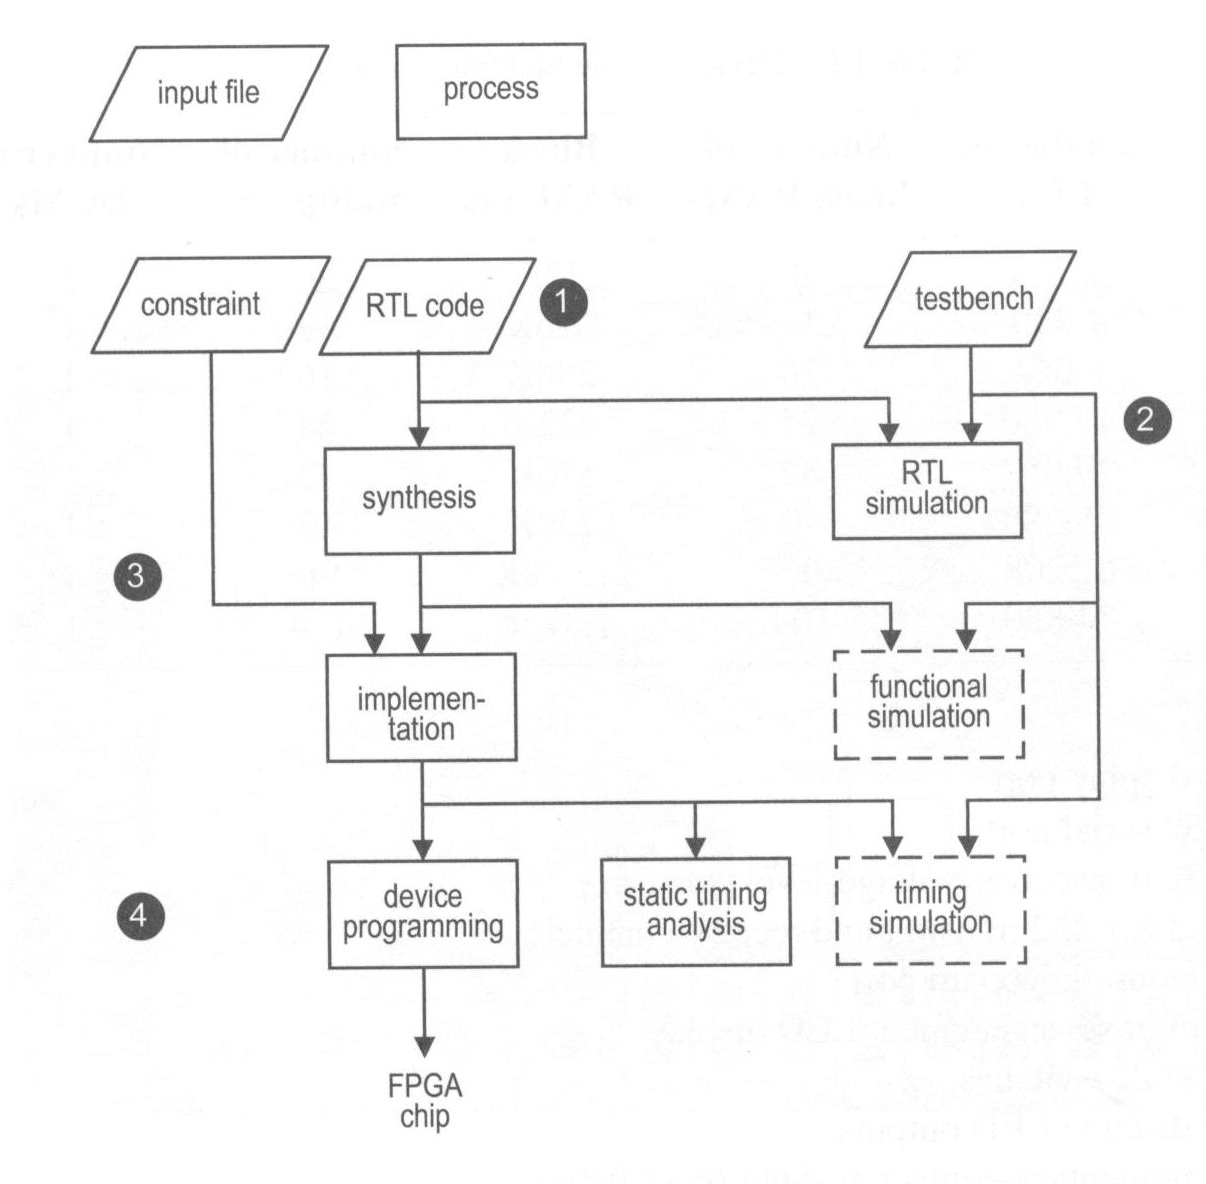
\includegraphics[width=0.5\textwidth]{pics/designprocess}
\end{center}

\subsection{Prozesse}
	\begin{itemize}
		\setlength{\itemsep}{1pt}
  	\setlength{\parskip}{0pt}
  	\setlength{\parsep}{0pt}
		\item Prozesse werden durch �nderungen an den Signalen in der Sensitivit�tsliste (im Prozess-Kopf) aktiviert und ausgef�hrt.
		\item Prozesse werden parallel abgearbeitet
		\item Innerhalb des Prozesses werden Anweisungen sequentiell abgearbeitet
		\item Selektive und konditionale Signalzuweisungen sind verboten.
		\item Unbedingte Signalzuweisung erlaubt. Aktualisierung aller Signale geschieht immer erst am Prozessende!
		\item G�ltig ist letzte Zuweisung
	\end{itemize}
	
	\lstinputlisting[language=vhdl,tabsize=2]{code/process.vhd}

\subsection{VHDL Code Example}
	\begin{center}
		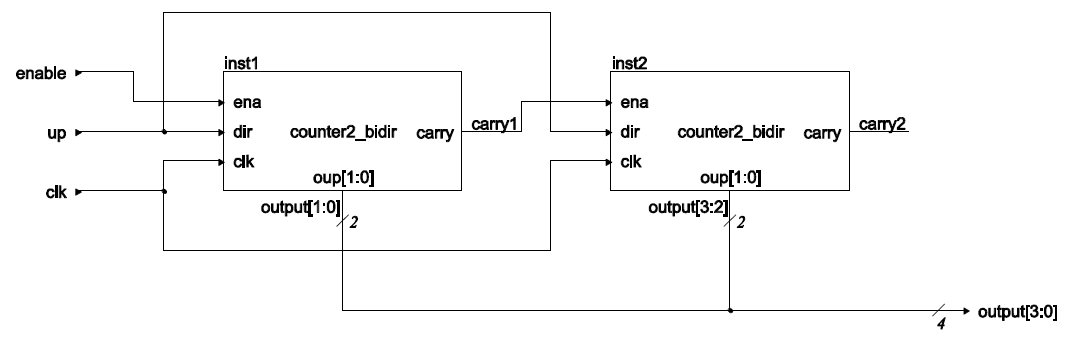
\includegraphics[width=0.5\textwidth]{pics/vhdlcodeexampleschematic.png}
	\end{center}
	\begin{multicols}{2}
		\lstinputlisting[language=vhdl,tabsize=2]{code/vhdlcodeexample.vhd}
	\end{multicols}